%!TEX TS-program = pdflatex or xelatex
%!TEX encoding = UTF-8 Unicode

\documentclass{article}
\usepackage[letterpaper, margin=1in] {geometry}
\usepackage{microtype} % micro appearance
\usepackage[all]{nowidow} % no lone lines
\usepackage{changepage} % changes layout mid-page
\usepackage{enumitem} % enum (itemize, enumerate, description)
\usepackage{ifthen}
\usepackage{xfrac}
\usepackage{fancyhdr} % headers
\usepackage{amsmath} % matrices
\usepackage{amssymb} % symbols
\usepackage{relsize}
\usepackage{gensymb} % symbols
\usepackage{tikz} % graphics?
\usepackage{bm} % bold math
\usepackage{multicol} % multiple columns
\usepackage{pgfplots}
\usepackage{lipsum} % lipsum
\usepackage{hyperref}
%\usepackage[compact]{titlesec}

\pagestyle{fancy}

\newcommand {\classname} {CS 4740/5740 -- Intro to Natural Language Processing}
\newcommand {\duedate} {Wed, 2014--04--30}
\newcommand {\hwtype} {Project}
\newcommand {\hwnum} {3 report}
\newcommand {\innermargin} {0.15in} % indentation amt of nested lst

\let\tss\textsuperscript
\let\oldunderline\underline
\renewcommand\underline[1]{\oldunderline{\smash{#1}}}

\fancyhead[L] {\ifthenelse {\thepage=1}
  {amw275 (Andy Wang), bgs53 (Ben Shulman),\\
   ms969 (MJ Sun), sg754 (Spandana Govindgari)}
  {\hwtype\ \hwnum\ (amw275, bgs53, ms969, sg754)}}
\fancyhead[R] {\ifthenelse {\thepage=1}
  {\classname\\\hwtype\ \hwnum\ (due \duedate)}
  {Page \thepage}}

\begin{document}
\begin{center}\textbf{Project 3: Report on Sequence tagging; Sentiment classification}\end{center}


\section{Introduction}
Our code is written in Python and Java. In this report we document how to classify sentiment at sentence level by implementing HMM and then experiment with different feature sets.


\section{Preprocessing}

\subsection{Configuration}
We implemented HMM as our sequence tagging system and did not use any existing Python libraries that provided implementations of HMMs. For experimenting purposes, we have looked at NLTK packages and for extracting features we decided use Chris Potts' interface to SentiWordNet.


\subsection{Data processing}
For pre-processing we have parsed \texttt{training\_data.txt} into memory using Python and NLTK. Our parser, \texttt{getReviewList}, returns a list of reviews whose sentences have been lemmatized and have removed stop words.

\begin{verbatim}
sentiment = strToSentiment(line[0]) # convert to 1,0,-1
sentence = utilities.cleanString(line[1]) # lemmatize and stopwords
lines.append((sentiment, sentence)) # collect as a tuple
\end{verbatim}


\section{Baseline}
We had two baseline measures. The first basline measure simply uses a random guess among the three states. While in the other baseline we recorded how many times each word occurs in a positive, neutral or negative sentence. Using that we estimated the probability of a sentence's sentiment. The code for this can be found in our baseline class in \texttt{baseline.py}.


\subsection{Model construction}
This class' constructor takes a source file where each review is separated by a newline, each sentence is tokenized and each on a separate line. Each sentence begins with its sentiment. Each review in the source file has its title on a line before its sentences. It also takes an \texttt{alpha} which is the add-alpha smoothing to use.

The constructor reads in the source file and then it maintains two counts as it goes over the file. It maintains \texttt{self.sentiment\_counts} which is a dictionary that holds the number of times each sentiment has appeared in the training set. It also maintains \texttt{self.word\_counts} which is a table (dictionary of dictionaries) with a row for each sentiment and a column for each token encountered. 

The constructor than iterates over all the sentences in the training set recording the number of times each sentiment occurs using \texttt{self.sentiment\_counts}. For each word in a sentence with sentiment \texttt{s} we add 1 to the value stored in \texttt{self.word\_counts[s][word]}. 

After going over all the training data the constructor then generates probabilities from the two tables. It generates entries for \texttt{self.sentiment\_probabilities} by simply using \texttt{self.sentiment\_counts} to calculate the probability of each sentiment occurring. Then for each column of the table, \texttt{self.word\_counts} we calculate the conditional probabilities $P(word|s)$ for all words and all sentiments and store them in \texttt{self.word\_probabilities}. After this our model has been constructed.


\subsection{Classification}
To classify a test set, one uses the \texttt{classify} function in the class. The function takes a \texttt{source} of the same form that the training data was. For each sentence in the test data we tag it with a sentiment using the following formula: $argmax_{s\in S}P(s)\mathlarger{\prod}_{w\in Sentence} P(w|s)$. In our code we use log probabilities to avoid underflow. Here is the code we use to tag each sentence:

\begin{verbatim}
                probs = dict()
                for sentiment in self.sentiment_probabilities:
                    probs[sentiment] = math.log(self.sentiment_probabilities[sentiment])
                for word in entry[1]:
                    if word in self.word_probabilities:
                        for p in self.word_probabilities[word]:
                            probs[p] += math.log(self.word_probabilities[word][p])
                tags.append(max(probs.iteritems(), key=operator.itemgetter(1))[0]
\end{verbatim}

We then write our predictions to a kaggle file, if define, as follows:
\begin{verbatim}
        if kaggle != None:
            with open(kaggle,'w') as f:
                f.write('Id,answer\n')
                i = 0
                for seq in predictions:
                    for tag in seq:
                        i += 1
                        f.write(str(i) + ',' + str(tag) + '\n')
\end{verbatim}

\subsection{Trivial baseline}
We also wrote a trivial baseline which simply guesses a random sentiment for each sentence, it is in \texttt{baseline\_random\_guess.py}


\section{Feature extraction}
Because of the limited number of examples we have for training, we need to represent the sentences using dense features that have many overlaps and don't produce a sparse matrix. As a result, we only use number of negative, neutral, and positive words to populate the feature vector. There are two basic variants of this approach. One is a basic counting scheme that gathers sentiment data only from the training set. The other retrieves sentiment scores from SentiWordNet 3.0.

\subsection{Basic sentiment labeling}
For the basic scheme, we look through the pre-processed training data, and create a dictionary that labels each word as positive, neutral, or negative. The way we calculate the sentiment of a word is by counting how many times it appears in a positive, neutral, or negative sentence, and the sentiment that the word appears in most becomes sentiment label of that word. If there is a tie, even if the tie is between positive and negative labels, the word is labeled neutral.

After going through the training data once to build this dictionary, we use it to count how many positive, neutral, and negative words a sentence has, and then normalize the count to get percentages. The three percentages become the feature vector representing this sentence. For test sets where sentences might contain words we have not previously seen in the training set, those words are labeled as neutral because that is the most common label. This representation is written out as \texttt{"basic\_features\_$[$test|train$]$.txt"}. 

We also want to see what would happen if we discard the unseen words in the test set, and if that would cause less bias towards neutral and improve the score. We write this representation out as:\\
\texttt{"basic\_features\_discard\_unseen\_$[$test|train$]$.txt"}.

\subsection{SentiWordNet labeling}
When just looking at the training data, we're limited by the words we've already seen. If a word we don't know appears in the test set, it doesn't help with representing the sentence. To maximize the contribution of words in a sentence, we decided to use sentiment labels for words from SentiWordNet 3.0. It is a sentiment tagger that is based off of WordNet 3.0. SentiWordNet has a positive, objective (equivalent to neutral in our case), and negative score for each synset from WordNet. The advantage of using SentiWordNet is that it labels many more words than our training data, but the disadvantage is that it is not specific to our corpus. Many words have different sentiments based on the context they're seen in, and SentiWordNet does not have that information. But we thought it would be interesting to compare the result of the two approaches.

To find the sentiment of a word, we use \href{http://compprag.christopherpotts.net/wordnet.html}{Christopher Potts}' SentiWordNet-Python interface (\texttt{sentiwordnet.py}) to extract all the synsets of the word and the positive, objective, and negative scores associated with the synsets. Since doing word sense disambiguation takes a long time and is also not always correct, we simply accumulate the scores of all the synsets and take the sentiment with the highest score as the label for that word. We then do the same procedure as for the basic feature extraction and calculate the positive, neutral, and negative score of each sentence. These features are labeled with \texttt{"sentiWordNet\_features\_binary"}.

\subsection{SentiWordNet scoring}
Since SentiWordNet gives us a score, and not just an integer value of positive, neutral, or negative, we can also use this information to enhance our feature vectors. Another variant to our SentiWordNet feature vector is that instead of each word contributing to either the positive, neutral, or negative count, we add the positive, neutral, and negative scores of each word provided by SentiWordNet to the overall score of the sentence, and then normalize afterwards. This gives a more accurate representation of how positive, neutral, and negative a sentence is. These features are labeled with \texttt{"sentiWordNet\_features\_score"}.

\subsection{Bucketing}
The sentiment scores of a sentence are all real number values. Since we need to match sentences to be able to productively use HMM and other methods, we need a way to group similar sentences. We are using bucketing to achieve this. For example, if the bucket size is 0.1, then if a sentence has positive score of [0.0, 0.1), we put it in bucket 1, if a sentence has positive score of [0.1, 0.2), we put it in bucket 2, so on and so forth. The features would become the bucket each score belongs to. Now we have three integer-valued features, and similar sentences would be grouped together when using HHM and other methods. The bucket size is a parameter we can tune. For the bucketed representation a \texttt{"bucket<bucketSize>"} label is added onto the text file names to identify them.


\section{Hidden Markov model}
We chose to implement our own Hidden Markov Model (HMM) along with experimenting with existing systems. To implement our HMM we created an HMM class in python.

\subsection{Model construction}
The constructor of the HMM takes a \texttt{source}, an \texttt{n}, a \texttt{beta} and an \texttt{alpha}. \texttt{source} is a string of the filename to use as training data. \texttt{n} is what n-gram the model will be (bigram, trigram, etc.), \texttt{alpha} is the add-k smoothing value to use for output counts and \texttt{beta} is the add-k smoothing value to use for transition counts. The constructor then parses the file to read create a list of reviews, \texttt{self.training\_data}. Each review in the resulting list is another list of tuples of the form \texttt{(sentiment,feature vector)}. Using this resulting data we generate a set of states, transition counts and output counts.

To generate the counts we use two dictionaries of dictionaries. The first is \texttt{self.output\_counts} which in each "row" has a state and each column is the sentence vector, thus \texttt{self.output\_counts[state][vector]} stores the number of times that vector appeared for that state. \texttt{transition\_counts} mean while, where each "row" is the previously seen \texttt{n-1} states and the column is the state being transitioned to. Thus \texttt{self.transition\_counts[previous][state]} stores the number of times state follows the \texttt{(n-1)-tuple} of previous states. As we go we also generate a set of all states: \texttt{self.states}.

We iterate over \texttt{self.training\_data} to generate the counts. For each review we iterate over the sentence tuples and for each sentence we add one to \texttt{self.output\_counts[state][vector]} for that sentence's vector and state. We also add one to the entry in  \texttt{self.transition\_counts[previous][state]} where \texttt{previous} is a tuple of the \texttt{(n-1)} previous states and \texttt{state} is the state for the sentence. We begin with the tuple \texttt{(start,)} as previous for the first sentence of each review. In order to account for potentially unseen vectors we create an entry in each state row for unknown with a count of 1. We chose not to use techniques such as replacing the first occurrence of each vector with an "unknown" one as we did in the first project due to the sparseness and small size of the training data. 

Using these counts we then generate the probability tables corresponding to the count tables by computing the conditional probability for each row by iterating over each row of each table.
 
\subsection{Classification and Viterbi}
To allow classification of test data we created two functions. The first is \texttt{classify} which takes in a source file and parses it into a list of reviews as was done in the model construction step. Then for each review (a list of sentence vectors) \texttt{classify} calls the function, viterbi, on that sequence. The function \texttt{viterbi} begins by initializing the necessary dynamic programming table, it then defines the base case (first column of the table). The base case is done by iterating over all states and finding the probability of transitioning from the start state to that state (\texttt{self.transition\_probabilities[('start',)][state]}) and then multiplying by the probability of emitting the first sentence vector from that state. Thus the code to do this is in our code is:
\begin{verbatim}
    (math.log(self.transition_probabilities[tuple(prev)][state])
        + math.log(self.output_probabilities[state][tuple(doc[0][1])])
\end{verbatim}

We use log probabilities throughout to avoid underflow. Afterwards we iterate over the rest of the sentences in the review. For each sentence in the review we iterate over all states and for each of those states iterate over every row in the dp table. This thus looks like this:
\begin{verbatim}
        for i in range(1,len(doc)):
            ...
            for state in self.states:
                ...
                for prev in table[0]:
                    ...
\end{verbatim}

In the innermost for loop we find the probability of transitioning from \texttt{prev} (in a bigram model this is simply a state, in a trigram it is 2 states) to \texttt{state}: this is \texttt{self.transition\_probabilities[prev][state]}.\par
We also find the probability of emitting the sentence vector at doc[i]:\\
\texttt{self.output\_probabilities[state][tuple(doc[i][1])]}.\par

We then also pull the entry for \texttt{prev} in the previous row: \texttt{table[i-1][prev][0]}.\par

We then do log addition to find the probability for this prev with this state for this sentence. Now for each \texttt{state} we take the maximum of all these calculated probabilities and do: \texttt{table[i][tuple(prev)] = (prob,trace)} where \texttt{prev} is now the the old prev plus the state, but retaining only the last n-1 states (so in trigram, you would retain the last state in prev and the new state to create the new prev). prob is the probability calculated and trace is the old prev, so we can trace back through the table at the end. We do this for all sentences and then trace back from the maximum value in the last column of the table to find the sequence of tags for this review. We then return the sequence of tags. 

The \texttt{classify} algorithm does this for every review, taking the returned lists and creating a list of lists, one list (sequence of tags) for each review. 

If we are writing our results to a kaggle-formatted file we do the following in our \texttt{classify} function: 
\begin{verbatim}
        if kaggle != None:
            with open(kaggle,'w') as f:
                f.write('Id,answer\n')
                i = 0
                for seq in predictions:
                    for tag in seq:
                        f.write(str(i) + ',' + str(tag) + '\n')
                        i += 1
\end{verbatim}

\subsection{Extension: n-gram HMM}
To support beyond a simple bigram HMM we implemented n-gram HMMs. The changes required for this were two-fold. First we had to change our model construction to keep track of more than one previous state (up to n-1 previous states instead) to construct our new transition counts, for instance each row of a transition matrix for a trigram HMM would be (1,1), (0,1), etc. for all combinations of states. 

We also had to change our viterbi algorithm to support n-grams. Much of how this works is detailed in the previous section, but instead of simply having the table have a row for every state we need to keep track of more than 1 previous state. Instead we keep track of n-1 previous states, for instance for a trigram we would have a row for ('start',1), (0,1), etc. Thus we don't actuall fill in every entry in a column for every column, we only fill in one per state, for instance (1,0), (1,1) and (0,2) would be filled because for each state we only take one maximum probability over all rows of the table and add that probability as one entry in the next column of the table.

\section{Experimentation}

Our procedures for experimentation involved the use of a bash shell script (\texttt{hmmexperiments}) that interacts with each train/test pairs generated from feature extraction and \texttt{hmm.py}, which uses our HMM implementation to guess positivity/neutrality.\par

For each train/test pair (as in \texttt{basic\_features\_train.txt} and \texttt{basic\_features\_test.txt}): we use our HMM to train on the training file, classify on the test file (or training file), and return a Kaggle-compliant CSV of results. This process is done for $n$-gram models from 2 to 4, various $\alpha$ and $\beta$ values (value for add-\texttt{alpha} and add-\texttt{beta} smoothing on ngram counts and transition counts, explained in above sections). \texttt{hmm.py} was formatted to take in the training file and find the corresponding test or training file to classify.\par

\begin{verbatim}
    for datafile in `ls data/basic_features_train.txt | sort`
    do  for ng in 2 3 4
        do  for alph in 0.01 0.05 0.1 0.5 1 1.5 2 3
            do  for bet in 0.01 0.05 0.1 0.5 1 1.3 2 2.2 2.5 3
                do
                    python ./hmm.py $datafile $ng $alph $bet
    done done done done
\end{verbatim}

Our baseline results on our test data (explained in previous sections):\par\medskip
\begin{tabular}{|c|c|}\hline
                        & precision\\\hline
Baseline                & \textbf{0.40196}\\
Baseline (random guess) & 0.32516\\\hline
\end{tabular}\par\medskip

It is expected that our random-guess baseline succeeds about a third of the time; there are three choices among pos/neu/neg. The reason our first baseline performs better than the random-guess baseline is that we take into account the frequency of words in positive / neutral / negative phrases, so that if we see a particular word that appears more frequently in one of the sentiments, we choose it and are more likely to succeed.

\par\bigskip
Our initial results on \emph{test data} (not training yet) are reported on the next page\ldots

\newpage
The following is a table of our experimental results generated by running \texttt{hmm.py} on our test data (explained in the above sections). For all results in the following table, $\alpha = \beta = 1$, the variables we use for add-\texttt{alpha} and add-\texttt{beta} smoothing (explained in the ``Model construction'' section above). The training data sets (and ``buckets'') used are also explained in sections above. Some of our best precisions per train/test feature pair are \textbf{bolded}.\par\bigskip

{\small
\begin{tabular}{|c|c|c|c|}\hline
Training data & bucket value & $n$-gram & Kaggle precision\\\hline
\texttt{basic\_features} & N/A (no bucketing) & 2 & \textbf{0.47059}\\\hline
\texttt{basic\_features} & N/A (no bucketing) & 3 & \textbf{0.46732}\\\hline
\texttt{basic\_features} & N/A (no bucketing) & 4 & \textbf{\textit{0.48039}}\\\hline\hline
\texttt{basic\_features\_discard\_unseen} & N/A (no bucketing) & 2 & 0.43954\\\hline
\texttt{basic\_features\_discard\_unseen} & N/A (no bucketing) & 3 & 0.44118\\\hline
\texttt{basic\_features\_discard\_unseen} & N/A (no bucketing) & 4 & 0.46732\\\hline
\texttt{basic\_features\_discard\_unseen} & 0.01 & 2 & 0.43301\\
\texttt{basic\_features\_discard\_unseen} & 0.05 & 2 & 0.44444\\
\texttt{basic\_features\_discard\_unseen} & 0.10 & 2 & 0.43301\\
\texttt{basic\_features\_discard\_unseen} & 0.20 & 2 & 0.44771\\\hline
\texttt{basic\_features\_discard\_unseen} & 0.01 & 3 & 0.44608\\
\texttt{basic\_features\_discard\_unseen} & 0.05 & 3 & \textbf{0.45915}\\
\texttt{basic\_features\_discard\_unseen} & 0.10 & 3 & 0.43791\\
\texttt{basic\_features\_discard\_unseen} & 0.20 & 3 & 0.44771\\\hline
\texttt{basic\_features\_discard\_unseen} & 0.01 & 4 & 0.45425\\
\texttt{basic\_features\_discard\_unseen} & 0.05 & 4 & \textbf{0.46569}\\
\texttt{basic\_features\_discard\_unseen} & 0.10 & 4 & 0.45261\\
\texttt{basic\_features\_discard\_unseen} & 0.20 & 4 & \textbf{0.46242}\\\hline\hline
\texttt{sentiWordNet\_binary} & 0.01 & 2 & \textbf{0.42157}\\
\texttt{sentiWordNet\_binary} & 0.05 & 2 & 0.40850\\
\texttt{sentiWordNet\_binary} & 0.10 & 2 & 0.39052\\
\texttt{sentiWordNet\_binary} & 0.20 & 2 & 0.33660\\\hline
\texttt{sentiWordNet\_binary} & 0.01 & 3 & \textbf{0.43137}\\
\texttt{sentiWordNet\_binary} & 0.05 & 3 & 0.40359\\
\texttt{sentiWordNet\_binary} & 0.10 & 3 & 0.33660\\
\texttt{sentiWordNet\_binary} & 0.20 & 3 & 0.31536\\\hline
\texttt{sentiWordNet\_binary} & 0.01 & 4 & \textbf{0.42810}\\
\texttt{sentiWordNet\_binary} & 0.05 & 4 & 0.41503\\
\texttt{sentiWordNet\_binary} & 0.10 & 4 & 0.37745\\
\texttt{sentiWordNet\_binary} & 0.20 & 4 & 0.34477\\\hline\hline
\texttt{sentiWordNet\_score} & 0.01 & 2 & 0.35294\\
\texttt{sentiWordNet\_score} & 0.05 & 2 & 0.39542\\
\texttt{sentiWordNet\_score} & 0.10 & 2 & \textbf{0.35948}\\
\texttt{sentiWordNet\_score} & 0.20 & 2 & 0.34477\\\hline
\texttt{sentiWordNet\_score} & 0.01 & 3 & 0.36765\\
\texttt{sentiWordNet\_score} & 0.05 & 3 & \textbf{0.38235}\\
\texttt{sentiWordNet\_score} & 0.10 & 3 & 0.35621\\
\texttt{sentiWordNet\_score} & 0.20 & 3 & 0.33170\\\hline
\texttt{sentiWordNet\_score} & 0.01 & 4 & 0.33170\\
\texttt{sentiWordNet\_score} & 0.05 & 4 & \textbf{0.38235}\\
\texttt{sentiWordNet\_score} & 0.10 & 4 & 0.33170\\
\texttt{sentiWordNet\_score} & 0.20 & 4 & 0.32516\\\hline
Training data & $n$-gram & bucket value & Kaggle precision\\\hline
\end{tabular}}\par\bigskip

We note that \texttt{basic\_features} without discarding performs the best (0.48039)! The fancy bucketing did not improve on our precision. We also note that SentiWordNet was not able to improve on these precisions either. This is probably because we have to consider context when determining whether a given word is positive, negative, or neutral, something that our usage of SentiWordNet does not perform adequately.\par

We can notice that a larger $n$-gram produced greater precisions: 4-grams were generally more precise than bigrams or trigrams. From these results, we attempted to experiment further with the training data derived only from basic features (the fact that using basic features with no discards with a 4-gram model performed the best).\par\bigskip

Here are some more of our results on test data, as we began experimenting with various smaller $\alpha$ values for less n-gram count smoothing. ($\alpha$ for add-\texttt{alpha} smoothing for n-gram output counts as explained above.) For all results in this table, we are using 4-gram, $\beta = 1$ (for add-\texttt{beta} smoothing). We also experimented with larger $\alpha$ for the basic features training/test pair:\par\bigskip

{\small\begin{tabular}{|c|c|c|c|}\hline
Training data & bucket value & $\bm{\alpha}$ & precision\\\hline
\texttt{basic\_features} & N/A (no bucketing) & 0.01 & \textbf{0.47386}\\
\texttt{basic\_features} & N/A (no bucketing) & \textbf{1.20} & \textbf{0.46078}\\
\texttt{basic\_features} & N/A (no bucketing) & \textbf{1.50} & \textbf{0.45752}\\
\texttt{basic\_features} & N/A (no bucketing) & \textbf{2.50} & \textbf{0.42801}\\\hline\hline
\texttt{basic\_features} & N/A (no bucketing) & \textbf{3.00} & \textbf{0.41503}\\\hline\hline

\texttt{basic\_features\_discard\_unseen} & N/A (no bucketing) & 0.01 & 0.44444\\
\texttt{basic\_features\_discard\_unseen} & 0.01 & 0.01 & 0.44444\\
\texttt{basic\_features\_discard\_unseen} & 0.05 & 0.01 & 0.44608\\
\texttt{basic\_features\_discard\_unseen} & 0.10 & 0.01 & 0.44118\\
\texttt{basic\_features\_discard\_unseen} & 0.20 & 0.01 & 0.46242\\\hline

\texttt{basic\_features} & N/A (no bucketing) & 0.05 & \textbf{0.47386}\\
\texttt{basic\_features\_discard\_unseen} & N/A (no bucketing) & 0.05 & 0.45261\\
\texttt{basic\_features\_discard\_unseen} & 0.01 & 0.05 & 0.45425\\
\texttt{basic\_features\_discard\_unseen} & 0.05 & 0.05 & 0.44935\\
\texttt{basic\_features\_discard\_unseen} & 0.10 & 0.05 & 0.44281\\
\texttt{basic\_features\_discard\_unseen} & 0.20 & 0.05 & 0.46078\\\hline

\texttt{basic\_features} & N/A (no bucketing) & 0.10 & \textbf{0.46732}\\
\texttt{basic\_features\_discard\_unseen} & N/A (no bucketing) & 0.10 & 0.46405\\
\texttt{basic\_features\_discard\_unseen} & 0.01 & 0.10 & 0.46405\\
\texttt{basic\_features\_discard\_unseen} & 0.05 & 0.10 & 0.45915\\
\texttt{basic\_features\_discard\_unseen} & 0.10 & 0.10 & 0.44118\\
\texttt{basic\_features\_discard\_unseen} & 0.20 & 0.10 & 0.46078\\\hline
\end{tabular}}\par\bigskip

We can conclude that $\alpha = 1$ yielded some of our most precise results: our previous best for \texttt{basic\_features} was \textbf{0.48039}. In light of these, we performed further experiments by fixing $\alpha$, and varying $\beta$. (4-gram, $\alpha = 1$ for \texttt{basic\_features})\par\bigskip

{\small\begin{tabular}{|c|c|c|c|c|c|c|c|c|c|c|c|c|c|c|}\hline
$\bm{\beta}$ & 0.01 & 0.1 & 0.7 & 1 & 1.2 & 1.8 & 2 & 2.5 & 3 & 5\\\hline
precision & .4673 & .4673 & .4673 & \textbf{.4804} & .4788 & .4788
& \textbf{.4820} & \textbf{.4820} & .4084 & .4576\\\hline
\end{tabular}}\par\bigskip

In summary, here are some of our \emph{best} results on \emph{test} data:\par\bigskip
\begin{tabular}{|c|c|}\hline
                           & precision\\\hline
Baseline                   & 0.40196\\
Baseline (random guess)    & 0.32516\\
Na\"{i}ve-Bayes classifier & 0.42320\\
HMM bigram, basic features, smoothing & 0.47059\\
HMM 3-gram, basic features, smoothing & 0.46732\\
HMM 4-gram, basic features, smoothing & \textbf{0.48203}\\\hline
\end{tabular}\par\medskip

We could have very likely achieved better precisions if we used MEMMs or CRFs. Our HMM implementation does not take context into consideration like CRFs, a modeling method that would perform very well in these classifications.

\subsubsection{Training precisions}
We also looked at our HMM's performance by checking the precision by using validation data: the training data itself. For this, we looked only at our best-performing feature data, \texttt{basic\_features} without discards, and without bucketing (with 2612 data points to work with). We varied the smoothing, and experimented with various $n$-grams.\par\medskip

{\small\begin{tabular}{|c|c|c|c|c|}\hline
$n$-gram & $\bm{\alpha}$ & $\bm{\beta}$ & \# correct &precision\\\hline
2 & 0.01 & 1 & 2092 & 0.80092\\
2 & 0.01 & 2 & 2094 & 0.80169\\
2 & 1    & 1 & 1910 & 0.73124\\
2 & 1    & 2 & 1910 & 0.73124\\
3 & 0.01 & 1 & 2088 & 0.79939\\
3 & 0.01 & 2 & 2090 & 0.80015\\
3 & 1    & 1 & 1893 & 0.72473\\
3 & 1    & 2 & 1898 & 0.72665\\
4 & 0.01 & 1 & 2114 & \textbf{0.80934}\\
4 & 0.01 & 2 & 2113 & \textbf{0.80896}\\
4 & 1    & 1 & 1907 & 0.73009\\
4 & 1    & 2 & 1909 & 0.73086\\\hline
\end{tabular}}\par\medskip

This data suggests that our HMM performs slightly better with a small amount of smoothing ($\alpha = 0.01$), that transition smoothing is not so effective, and that each $n$-gram model performs very similarly. Our best-performing model is a 4-gram with not so much smoothing on counts (precision of 0.80934). This data \emph{agrees} with our finding that our HMM performs better with bigrams than trigrams as well! (Precisions from test data on \texttt{basic\_features} is greater on bigrams than trigrams.)

\subsection{Error analysis}
Our system works well when there is a large training set and when the training corpus is of the same style as the input to be classified. This is evident from the fact that our accuracies on training set was nearly double the accuracies we got when we used the test set. However, there were times when the system did not work well and the following could be reasons why it did not perform as well: 
\begin{enumerate}
\item Most of our errors have resulted from the limited coverage that the training data gave. We also failed to take into account sarcasm, false positives and false negatives.
\item Some errors were due to complex, long and unusual sentence structure, which our simple feature encoding did not capture well.
\item False positives:
  \begin{enumerate}[nolistsep,noitemsep]
    \item \textit{I am returning the unit to the store and looking for a \emph{better} replacement.}
    \item \textit{To teach Middle Eastern dance in any form---a real dance video, or an exercise video---you should know how to do it yourself.}
  \end{enumerate}
  In the first example, better is annotated as positive therefore, making the entire sentence positive. In this case, context plays an important role since returning conveys negative connotation. We did not take into account context like CRFs do, therefore, HMM marked this as positive. And in the second example, the sentence has a sarcastic sense. Since our system did not take into account such instances, it marked the phrase positive. 
\item False negatives:
  \begin{enumerate}[nolistsep,noitemsep]
  \item \textit{First I become exposed to his brilliance via I Got You, the break through song of Split Enz a quarter of a century ago.}
  \end{enumerate}
  The phrase ``break through'' was annotated here as negative which made the entire sentence to be tagged as negative. The primary reason here was due to the limited coverage of our training data. Many words in this sentence were unseen and proper nouns. We did not take into account capitalization as one of our feature which here could helped us identify sentiment.

\item Long and complex sentence structures
    \begin{enumerate}
    \item \textit{[pos] However, I do not recommend this, because the softy in me found myself tearing up on a few occasions and     trying to fight back the tears as other people trying to get to work pretended not to notice.      
    }
    \item \textit{[neg] I can create play lists in Windows Media Player on my desktop and when I connect the Treo using the USB     cable my play lists are automatically synced to the storage card.}
\end{enumerate}
The above sentences were wrongly predicted to be positive/negative as both the sentences are long and complex.
\end{enumerate} 
To improve the system we added smoothing, worked with different n-gram models and smoothed the HMM transitions. What helped the most was a higher n-gram model. We also improved the existing systems by extracting other feature sets by bucking and sentiWordNet. None of these helped improve our current model since we performed the best with basic features. Our system could be further improved by extracting other features like capitalization, taking into account the polarities of context words, using better models like CRFs and MEMMs.
\section{Final Kaggle score}
Our Kaggle team is \textbf{abms}.\par
For our two submissions, we are officially counting two csvs generated from our HMM implementation with a 4-gram model, with smoothing on both n-gram counts and HMM transition counts. For $\beta = 1$, we received a score of \textbf{0.48039}. For $\beta = 2$, we received a score of \textbf{0.48203}.\par\medskip

\noindent
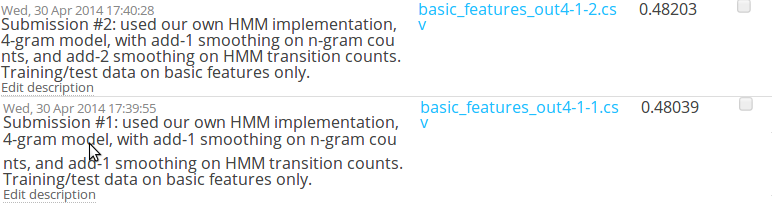
\includegraphics[width=\textwidth]{kagglesubs.png}\par\bigskip

\section{Member contributions}
\begin{itemize}[noitemsep]
  \item MJ Sun: feature extraction
  \item Ben Shulman: HMM implementation, baseline, and extension
  \item Andy Wang: HMM experimentation
  \item Spandana Govindgari: experimentation with packages
\end{itemize}
\end{document}
